\section{Training and evaluation}
\label{sec:protocol}

\subsection{Grouped out-of-fold training and final refitting}

Five rotations of eight-sequence blocks generate leakage-controlled inputs for the upper stages. In each rotation, twenty-four groups fit the four producers and two PAIR heads, eight different groups fit the context refiners and normalizers, and the remaining eight groups generate out-of-fold features. A query group never contributes to supervised fitting of the models that generate its upper-stage features. \evidence{M23}

We pool PHASE17 RGB and event features across the out-of-fold rotations to train the context heads and normalizers. Those models then generate the PHASE20 features, expressed through the 340-coordinate container, for fusion-head training. Rotations pool named fields with shared semantics, while learned hidden coordinates stay within their originating models. Targets join the data only after out-of-fold feature generation. \evidence{M23}

\begin{figure}[htbp]
\centering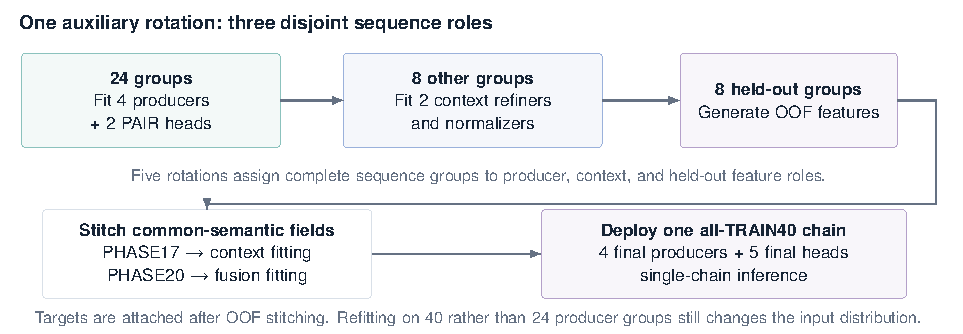
\includegraphics[width=\linewidth]{figures/rev_oof.pdf}
\caption{\textbf{Five-rotation fitting scheme.} Each rotation separates producer fitting, context fitting, and held-out feature generation. Final refitting produces one all-TRAIN40 inference chain. \evidence{M23}}
\label{fig:oof}
\end{figure}

Inference executes one all-TRAIN40 chain comprising the four producers, two PAIR heads, two context refiners, and fusion head. Auxiliary producers see twenty-four groups per rotation, whereas deployed producers see all forty. This stage-wise exposure difference can shift the upper-stage feature distribution after refitting. Earlier development use also remains relevant to architecture-selection claims.

Training comprised 690,934 auxiliary endpoint updates and 58,660 final-head updates across forty-five fits. Final PAIR endpoints used 11,264 updates; each context model and the final head used 12,044. Schedulers and warmup scaled with the fitting population. Update counts describe optimization exposure rather than wall-clock GPU effort. \evidence{L45}

Producer training combines relational DINO teacher signals, foreground geometry supervision, and task-specific adaptation. The deployed chain no longer evaluates the generic teacher, but its supervision remains part of the training recipe.


\subsection{Metrics and target coordinates}
TTC error in seconds, inverse-TTC error, benchmark phase error, and detection of urgent risk measure different aspects of behaviour. We use the signed benchmark phase
\begin{equation}
\phi(T)=-\log\!\left(1-\frac{0.1\,\mathrm{s}}{T}\right),\qquad T<0\;\text{or}\;T>0.1\,\mathrm{s}.
\end{equation}
Negative TTC denotes recession. The interval $[0,0.1]$\,s is outside this transform's domain. The official benchmark scorer defines motion-in-depth (MiD) error as
\begin{equation}
 \mathrm{MiD}(\widehat T,T)=10^4\left|\log\left(1-\frac{0.1}{T}\right)
 -\log\left(1-\frac{0.1}{\widehat T}\right)\right|
 =10^4|\phi(\widehat T)-\phi(T)|.
\end{equation}
MiD measures phase displacement. At large positive $T$, the first-order approximation $\phi(T)\simeq0.1/T$ compresses differences in seconds, while sensitivity rises near the positive domain boundary. We therefore report MAE in seconds alongside MiD. \evidence{M10,M15}

The scorer groups target TTC into four right-closed intervals: crucial $c:(0,3]$\,s, small $s:(3,6]$\,s, large $l:(6,10]$\,s, and negative $n:(-10,0]$\,s. The grouping includes zero in the negative band, although the phase transform is undefined at zero; metric validity is checked separately. Targets outside these bands do not contribute to the band-weighted score.

The scorer computes the band-weighted score
\begin{equation}
 \mathrm{overall\_MiD}=0.5\,\mathrm{MiD}_{c}+0.3\,\mathrm{MiD}_{s}
                     +0.1\,\mathrm{MiD}_{l}+0.1\,\mathrm{MiD}_{n},
\end{equation}
and a sample-weighted mean MiD. Missing bands remain missing, without weight redistribution. The complete band-weighted score requires targets in all four bands. The evaluation fixes the scorer by SHA-256 and tests a perfect four-band example, a hand-computed crucial-band error, and an absent negative band. \evidence{M15}

Metric reductions retain failures explicitly. The wrapper records invalid predictions by band and leaves its strict mean unavailable when any row is invalid. The official failure rate differs from the false-negative rate for urgent collision warnings. We therefore report prediction coverage, invalid-MiD count, and risk recall with their respective metrics. A finite saturated TTC may still carry an unsupported-measurement flag.

\subsection{Official benchmark and exploratory evaluations}

\begin{table}[H]
\centering\small
\caption{Evaluation populations and the quantities each supports. Historical46 and Extended-new share three sequence groups but no query identities.}
\label{tab:evaluation-populations}
\begin{tabularx}{\linewidth}{@{}>{\raggedright\arraybackslash}p{.24\linewidth}>{\raggedright\arraybackslash}p{.22\linewidth}X@{}}
\toprule Population & Size & Interpretation \\\midrule
Official GarlTTC Test & 6,762 scored tokens & Private targets; band-weighted MiD and scorer-defined failures. \evidence{B01,B02} \\
Published Garl EvTTC & 3 sequences & Published RTE; target/query correspondence to our run unverified. \evidence{T02} \\
EvTTC competition & 434 queries; 10 sequences & Unscored predictions, coverage and disagreement. \evidence{T01} \\
EvTTC Extended-new & 468 targets; 32 sequences & Labeled, development-exposed transfer with annotated ROI. \evidence{L01} \\
EvTTC Historical46 & 46 targets; 3 sequences & Labeled, development-exposed transfer with annotated ROI. \evidence{L01} \\
\bottomrule\end{tabularx}
\end{table}


The official GarlTTC Test submission covers twelve sequences and uses TRAIN40 event--RGB inputs with up to 650\,ms of causal history. Section~\ref{sec:official} reports the public ranking as of 28 October 2026 over \OfficialSampleCount{} scored tokens, including aliases of repeated physical queries \citep{codabench2026}. The evaluator scores submitted TTC values without standardizing temporal support, localization, supervision, or runtime across systems. Separate development experiments probe mechanisms within their tested configurations. \evidence{B01,B02,L44}

\subsection{Independence and paired comparisons}
Complete sequences form the units of separation and resampling. A sample-weighted sequence bootstrap carries all rows from each sampled group into the replicate and recomputes the ratio of summed losses to summed counts; sequence-macro summaries weight groups equally. Both reductions inherit any development exposure. Appendix~\ref{app:evaluation-details} gives the corresponding lineage, causality, and latency checks. \evidence{M15--M20}

Three head seeds quantify optimization variability conditional on their parents; they do not independently replicate the upstream representation. The additional transfer bootstrap is post hoc: it resamples saved paired predictions without changing a model, split, or historical interval (Appendix~\ref{app:derived-transfer}).
\FloatBarrier
